%---------------Preamble---------------------
\documentclass{beamer}

% Theme and color
\usetheme{Madrid}
%\usetheme{Pittsburgh}
\usefonttheme{serif}
%\usecolortheme{default}
\usecolortheme{seahorse}
\setbeamertemplate{itemize items}[ball]

% Addtional Packages
\usepackage{listings}
\usepackage{algorithm}
\usepackage{algpseudocode}
\usepackage{xcolor}
\usepackage{caption} % captions in tables
\usepackage{graphicx} % images

% Styling python code globally
\lstdefinestyle{pythonstyle}{
  language=Python,
  backgroundcolor=\color{white},
  commentstyle=\color{green!40!black},
  keywordstyle=\color{blue},
  numberstyle=\tiny\color{gray},
  stringstyle=\color{purple!60!black},
  basicstyle=\ttfamily\footnotesize,
  breakatwhitespace=false,
  breaklines=true,
  captionpos=b,
  keepspaces=true,
  numbers=left,
  numbersep=5pt,
  showspaces=false,
  showstringspaces=false,
  showtabs=false,
  tabsize=2
}
\lstset{style=pythonstyle}

% Title details
\title{Reinforcement Learning for Pseudo-Labeling}
\subtitle{Capstone Project Presentation}
\author{
  Group-11
  \\
  \vspace{0.3cm}
  \textbf{Students:} Aishwarya Maddula, Deepika Reddygari, Phanindra Kalaga, Prudhvi Chekuri
  \\
  \vspace{0.3cm}
  \textbf{Guided by:} Dr. Amir Jafari, Prof. Tyler Wallett
}
\institute{George Washington University}
\date{}

% Footer Details
\setbeamertemplate{footline}{
  \leavevmode
  \makebox[\linewidth]{%
    \hspace{0.5cm}%
    \scriptsize \insertshorttitle%
    \hfill%
    \scriptsize \insertframenumber/\inserttotalframenumber \hspace{0cm}%
  }%
  \vspace{0.2cm}
}
%---------------Document---------------------

\begin{document}

%--------------------------

\begin{frame}
  \titlepage
\end{frame}

%--------------------------

\begin{frame}{Outline}
  \tableofcontents
\end{frame}

%--------------------------

\section{Introduction}
\begin{frame}{Introduction}
  \begin{itemize}
    \item \textbf{Problem:} Labeled data is limited and costly to obtain.
      \\~\\
    \item \textbf{Challenge:} Traditional pseudo-labeling often propogates errors.
      \\~\\
    \item \textbf{Idea:} Use Reinforcement Learning (RL) to adaptively select pseudo-labels and improve error rate.
  \end{itemize}
\end{frame}

%--------------------------

\section{Background and Literature Review}
\begin{frame}{Background and Literature Review}
  \begin{itemize}
    \item The team began with introductory RL implementations using examples from the \texttt{gymnasium} library to build foundational understanding. \\~\\
    \item Conducted an initial review and implementation of five RL-based pseudo-labeling studies to establish a research baseline. \\~\\ \\~\\
      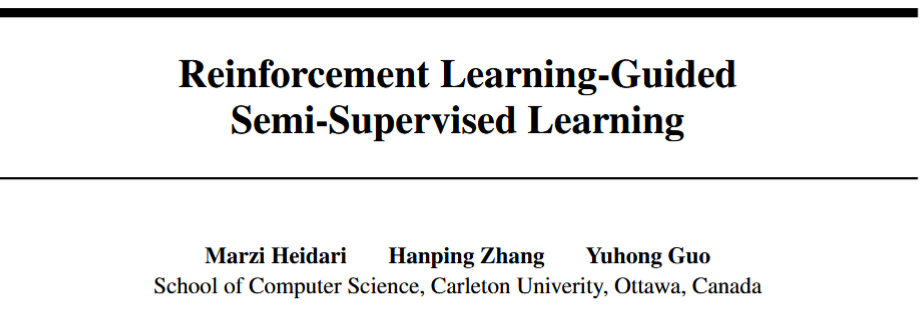
\includegraphics[width=0.32\linewidth]{RLPL/images/RLGSSL.png}
      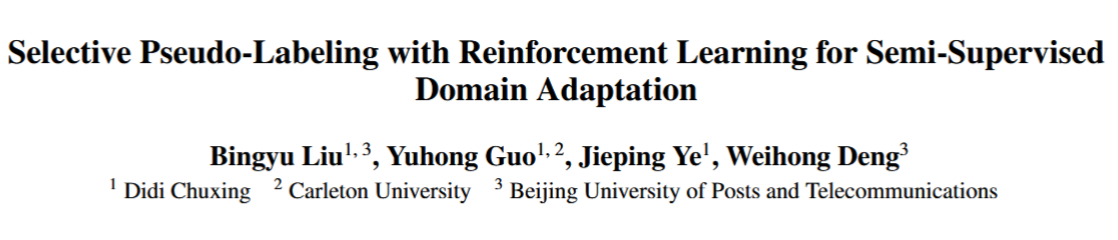
\includegraphics[width=0.32\linewidth]{RLPL/images/2012-03438.png}
      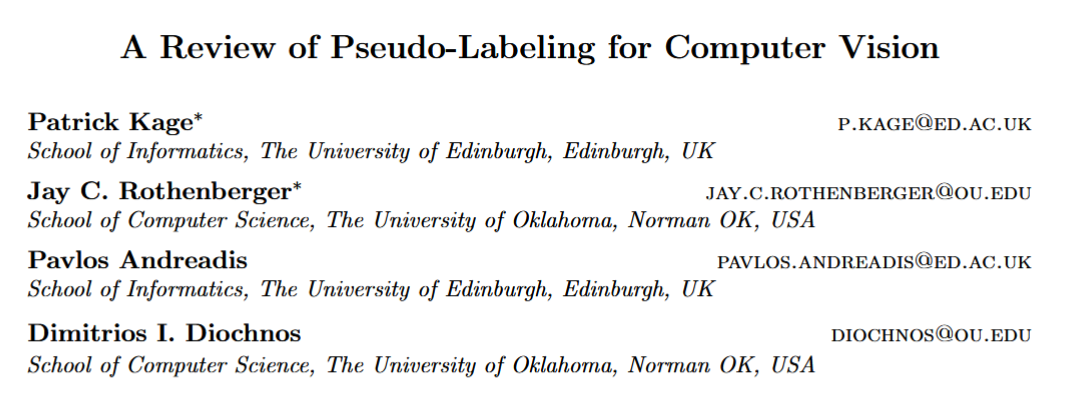
\includegraphics[width=0.32\linewidth]{RLPL/images/2408-07221.png}

  \end{itemize}
\end{frame}

%--------------------------

\section{Reinforcement Learning Framework}

\begin{frame}{Reinforcement Learning Introduction}
  \begin{columns}[T]
    \begin{column}{0.6\textwidth}
      \begin{itemize}
        \item \textbf{Reinforcement Learning:} Agent learns through interaction and feedback from the environment. \\~\\
        \item \textbf{Sequential Decision Making:} Each action affects future states and rewards. \\~\\
        \item \textbf{Markov Decision Process (MDP):} Framework for modelling decision making.
      \end{itemize}
    \end{column}

    \begin{column}{0.4\textwidth}
      \centering
      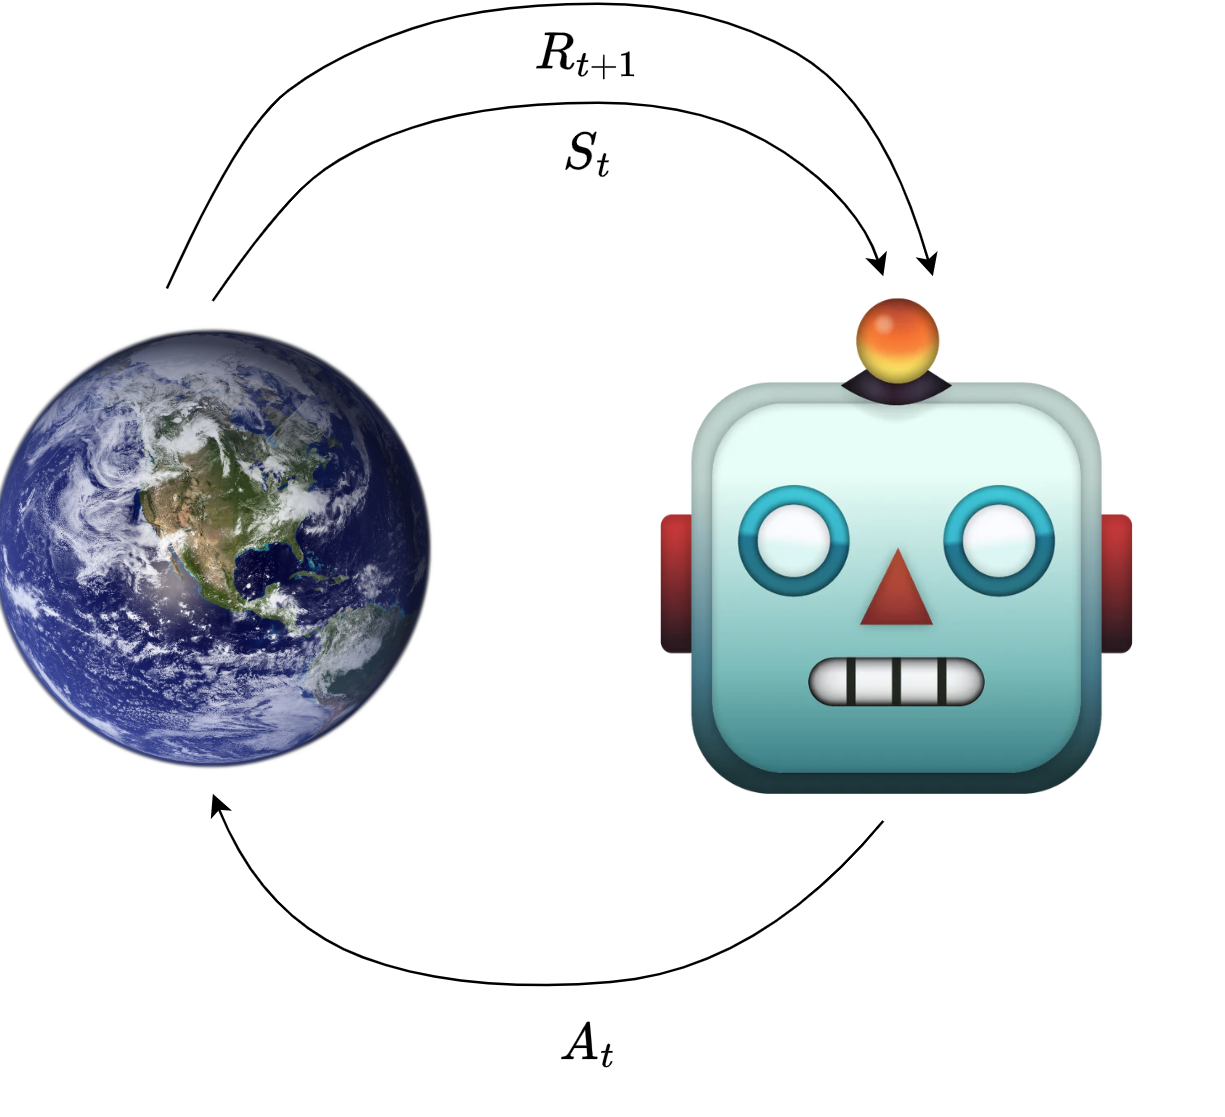
\includegraphics[width=\linewidth]{RLPL/images/MDP.png} \\[0.3em]
      {\small\textbf{Markov Decision Process}}
    \end{column}
  \end{columns}
\end{frame}

%--------------------------

\begin{frame}
  \centering 
  \large Approach-1 \\~\\
  \large Reinforcement Learning Using Policy Gradient
\end{frame}

%--------------------------

\begin{frame}{MDP Formulation}
  \begin{block}{State}
    Image features, model predictions, entropy (uncertainty).
    \begin{center}
      $\mathcal{S} = \{ \mathbf{X} ; \ \text{softmax}(\mathbf{y}) ; \ \mathcal{L}  \}$
    \end{center}
  \end{block}
  \begin{block}{Action}
    Assign pseudo-label or skip.
    \begin{center}
      $\mathcal{A} = \{ 0, \ldots, 9, ; \ \text{skip} \}$
    \end{center}
  \end{block}
  \begin{block}{Reward}
    Error Rate improvement of downstream model on validation data.
    \begin{center}
      $\mathcal R_{t} = -(e_{t} - e_{t-1})$
    \end{center}
  \end{block}
\end{frame}

%--------------------------

\section{Project Setup}
\begin{frame}{Code Files}
  \begin{itemize}
    \item \textbf{main.py}: Entry point for training process.
    \item \textbf{env.py}: Custom RL environment handling pseudo-labeling episodes.
    \item \textbf{model.py}: Updates policy based on agent's actions for maximising reward.
    \item \textbf{utils.py}: Helper functions for data loading, metrics, etc.
  \end{itemize}
  \centering
  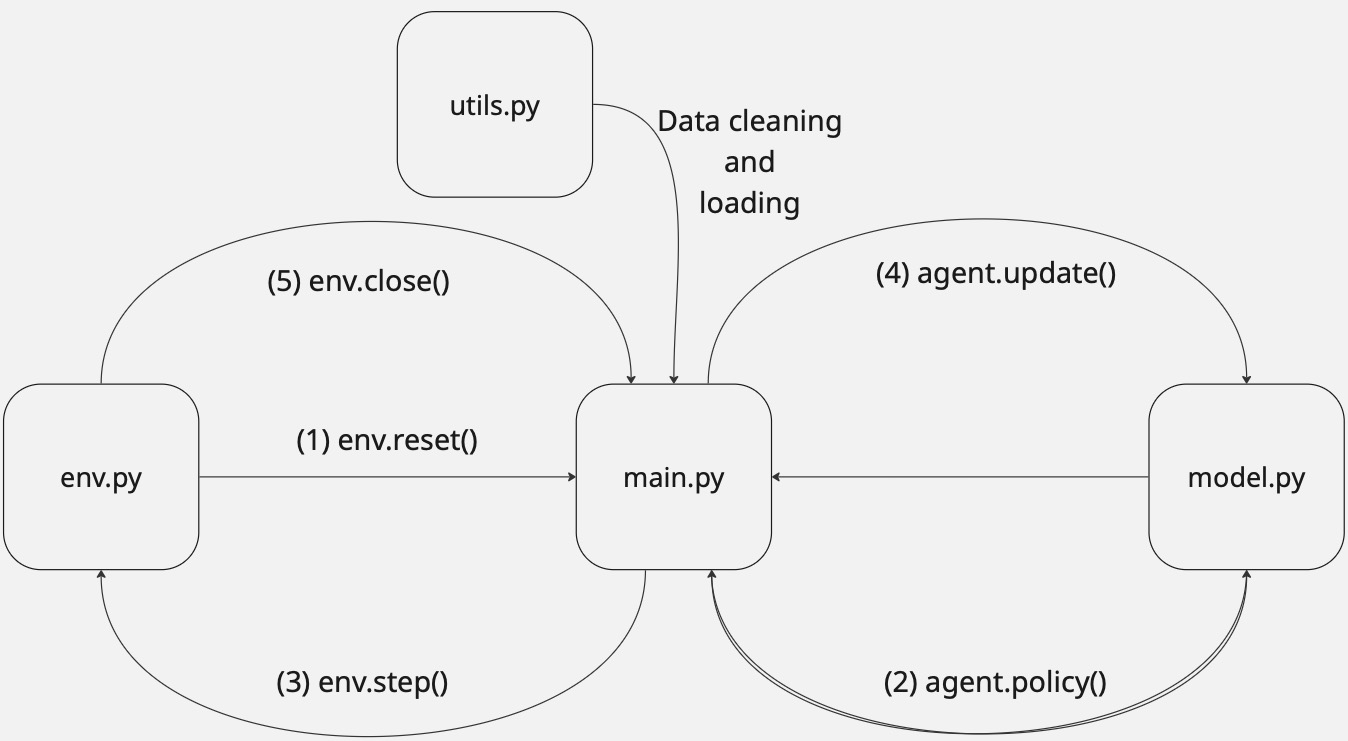
\includegraphics[width=0.7\linewidth]{RLPL/images/workflow.jpg} \\
\end{frame}

%--------------------------
\begin{frame}{Flow Diagram}
  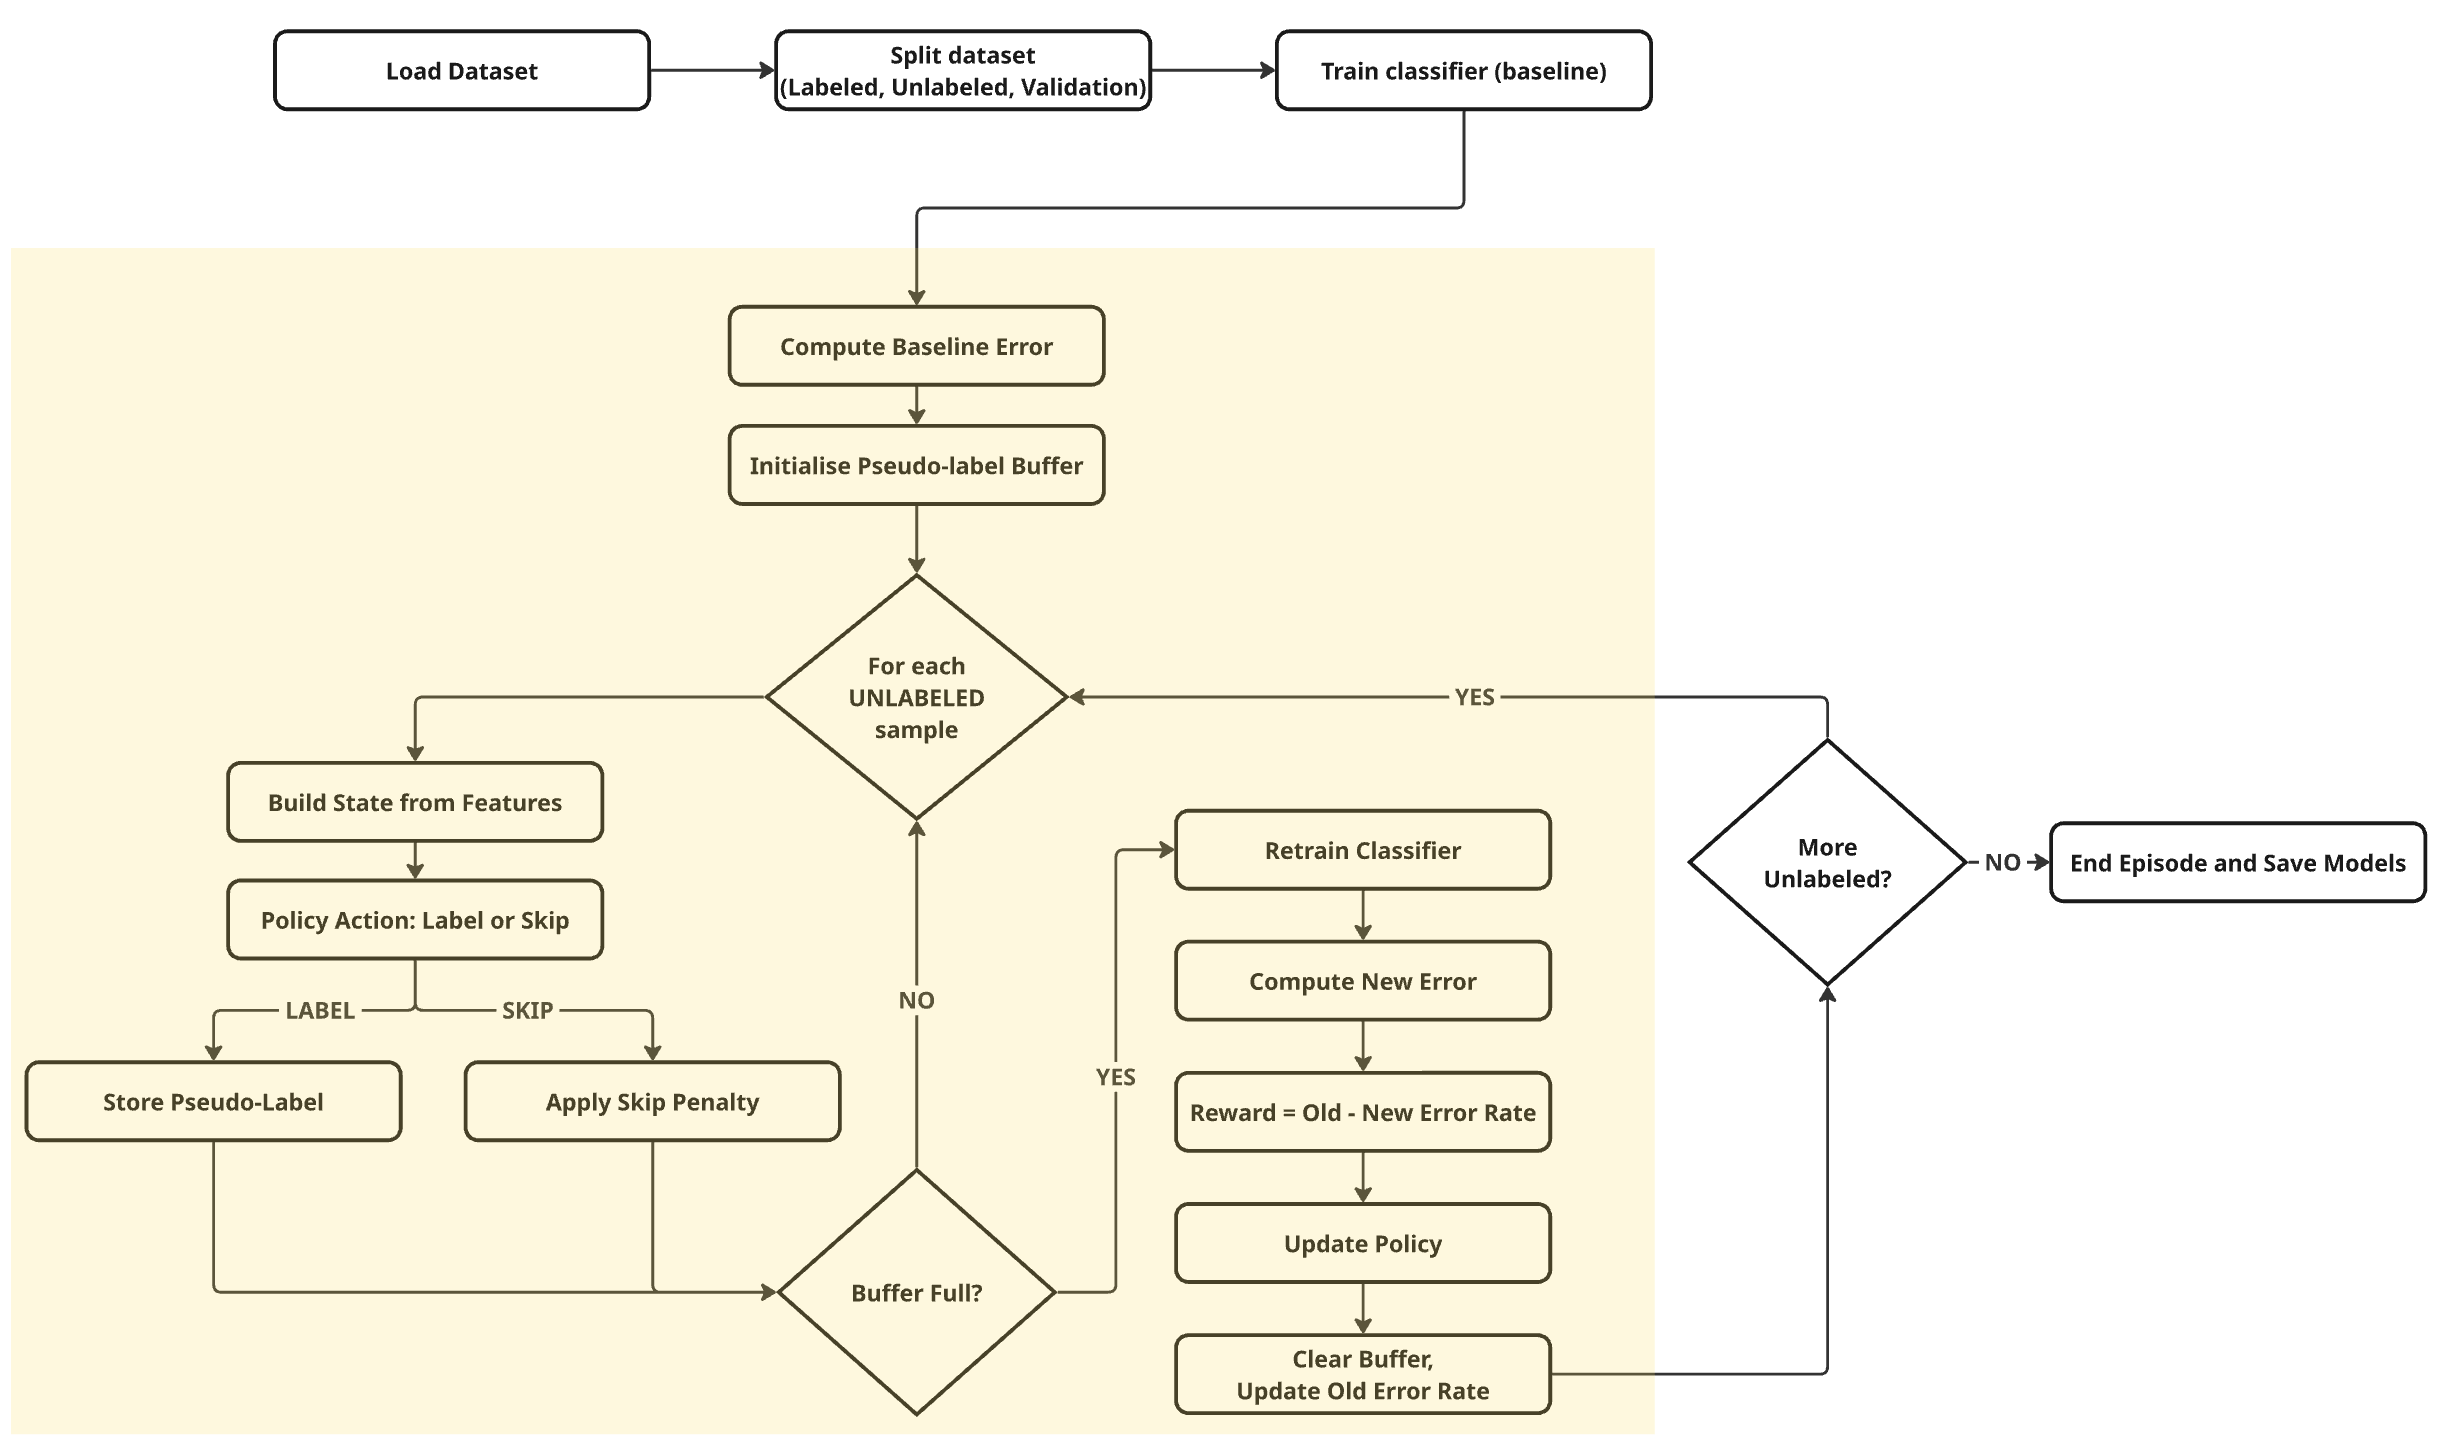
\includegraphics[width=1.0\linewidth]{RLPL/images/Flow_Diagram.png} \\
\end{frame}
%--------------------------

\section{PseudoCode}
\begin{frame}{PseudoCode}
  \begin{algorithm}[H]
    \caption{RL agent training loop}
    \label{alg:rl_training_algpseudocode}
    \scriptsize
    \begin{algorithmic}
      \Require state\_dim, action\_dim, labeled\_data, unlabeled\_data, num\_episodes
      \State agent $\leftarrow$ \texttt{RLAgent}(state\_dim, action\_dim)
      \State env $\leftarrow$ \texttt{PseudoLabelEnv}(labeled\_data, unlabeled\_data) \\~\\
      \For{episode = 1 \textbf{to} num\_episodes}
      \State state $\leftarrow$ env.reset()
      \State done $\leftarrow$ false
      \While{not done}
      \State action $\leftarrow$ agent.select\_action(state)
      \State $(\text{next\_state},\ \text{reward},\ \text{terminated},\ \text{info}) \leftarrow \text{env.step(action)}$
      \State state $\leftarrow$ next\_state
      \State done $\leftarrow$ terminated
      \EndWhile
      \State agent.update()
      \State error rate $\leftarrow$ env.evaluate()
      \EndFor
      \State env.close()
    \end{algorithmic}
  \end{algorithm}
\end{frame}

%--------------------------

\section{Implementation Details}

\begin{frame}[fragile]{env.reset()}
  \begin{itemize}
      \lstinputlisting[basicstyle=\ttfamily\fontsize{5.5}{7.5}\selectfont,firstline=72, lastline=87]{RLPL/env.py} \\~\\
    \item \textbf{Input:} Random seed and options. \\~\\
    \item \textbf{Functionality:} Resets the environment. \\~\\ %by
    \item \textbf{Output:} Initial environment state and empty info dictionary.
  \end{itemize}
\end{frame}

%--------------------------

\begin{frame}{model.policy()}
  \lstinputlisting[basicstyle=\ttfamily\fontsize{5.5}{7.5}\selectfont, firstline=408, lastline=408]{RLPL/model.py}
  \lstinputlisting[basicstyle=\ttfamily\fontsize{5.5}{7.5}\selectfont, firstline=418, lastline=423]{RLPL/model.py} \\~\\
  \begin{itemize}
    \item \textbf{Input:} Current state ($S_{t}$).\\~\\
    \item \textbf{Functionality:} Action (pseudolabel) is selected based on logits obtained from policy network.
      \begin{center}
        $a \in \mathcal{A}(s)$
      \end{center} \\~\\
    \item \textbf{Output:} Selected action as integer.
  \end{itemize}
\end{frame}


%--------------------------

\begin{frame}{env.step()}
  \lstinputlisting[basicstyle=\ttfamily\fontsize{5.5}{7.5}\selectfont, firstline=92, lastline=118]{RLPL/env.py}
\end{frame}

\begin{frame}[fragile]{env.step()}
  \begin{itemize}
    \item \textbf{Input:} Action selected by the agent.  \\~\\
    \item \textbf{Functionality:} There are multiple functionalities like: \\~\\
      \begin{itemize}
        \item Computes reward based on prediction and action.
        \item Updates pseudo-labeled data.
      \end{itemize} \\~\\
    \item \textbf{Output:} Returns next state, total reward, termination flag, and performance info (error rate, final reward).
  \end{itemize}
\end{frame}

%--------------------------

\begin{frame}{model.update()}
  \lstinputlisting[basicstyle=\ttfamily\fontsize{5.5}{7.5}\selectfont, firstline=460, lastline=485]{RLPL/model.py}
\end{frame}

\begin{frame}[fragile]{model.update()}
  \begin{itemize}
    \item \textbf{Input:} Sampled states, actions, and rewards from agent experience. \\~\\
    \item \textbf{Functionality:} There are multiple functionalities like: \\~\\
      \begin{itemize}
        \item Computes advantages using rewards-to-go and value estimates.
        \item Updates policy network ($\pi_{\theta}(a|s)$) to maximize expected reward.
        \item Updates value network ($V^{\pi}_{\theta}$) to minimize prediction error.
      \end{itemize} \\~\\
    \item \textbf{Output:} Returns policy loss and value loss for performance tracking.
  \end{itemize}
\end{frame}

%--------------------------

\begin{frame}{main.py (Bringing everything together)}
  \lstinputlisting[basicstyle=\ttfamily\fontsize{5.5}{7.5}\selectfont, firstline=10, lastline=38]{RLPL/main.py}
\end{frame}

%------------------------------

\section{Results and Insights}
\begin{frame}{Key Observations}
  \begin{itemize}
    \item CNN benefits more from RL guidance than ResNet due to weaker baseline.
    \item Performance degradation observed after multiple episodes.
    \item \textbf{Key Bottleneck:} Reward design and confirmation bias.
  \end{itemize}

  \vspace{0.3cm}
  \renewcommand{\arraystretch}{1.3}
  \centering
  \begin{table}[h]
    \centering
    \begin{tabular}{lcc}
      \hline
      \textbf{Model} & \textbf{MNIST} & \textbf{CIFAR-10} \\
      \hline
      CNN      & 3.45\%  & 34.40\% \\
      MLP      & 37.40\% & 59.60\% \\
      ResNet18 & 5.80\%  & 25.75\% \\
      \hline
    \end{tabular}
    \caption{Performance comparison on MNIST and CIFAR-10}
  \end{table}

  \vspace{0.2cm}
  \captionof*{table}{\textbf{Final Classification Error rate Comparison}}
\end{frame}

% ----------------------------

\begin{frame}
  \centering
  \large Approach-2 \\~\\
  \large Reinforcement Learning Guided Semi-Supervised Learning \\(RLGSSL) \\~\\
  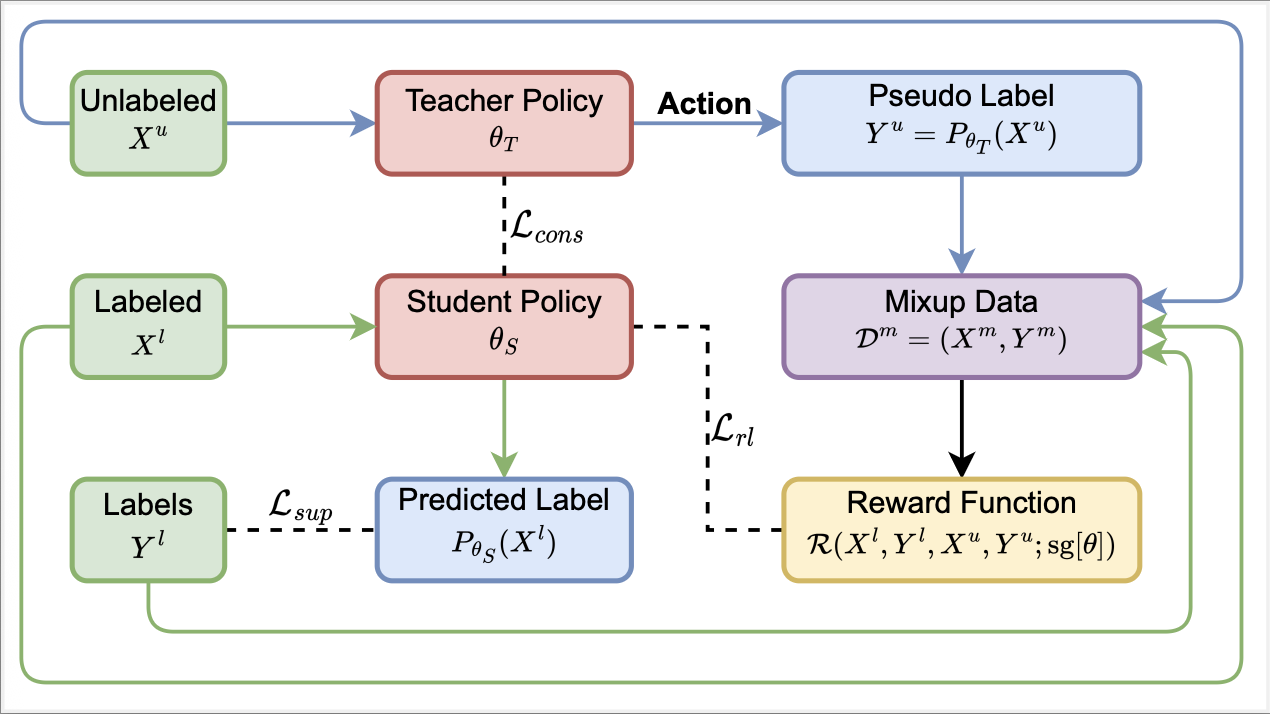
\includegraphics[width=0.7\linewidth]{RLPL/images/RLGSSL_titleimage.png}
\end{frame}

%--------------------------
\section{PseudoCode RLGSSL}
\begin{frame}{PseudoCode RLGSSL}

\begin{algorithm}[H]
\caption{RL-Guided SSL}
\scriptsize
\begin{algorithmic}

\Require $\mathcal{D}^l$, $\mathcal{D}^u$, and extended $\widetilde{\mathcal{D}}^l$; initialized $\theta_S$, $\theta_T$; hyperparameters

\For{iteration $= 1$ to maxiters}

    \For{each $x_i^u \in \mathcal{D}^u$}
        \State Compute soft pseudo-label vector $y_i^u = P_{\theta_T}(x_i^u)$ to form $(x_i^u, y_i^u)$
    \EndFor

    \State Generate mixup data $\mathcal{D}^m = (X^m, Y^m)$ on $\mathcal{D}^u$ and $\widetilde{\mathcal{D}}^l$ using with shuffling

    \For{step $= 1$ to maxsteps}
        \State Draw a batch of data $B = \{(x_i^m, y_i^m)\}$ from $\mathcal{D}^m$
        \State Calculate the reward function $\mathcal{R}(\cdot ; sg[\theta_S])$ using the batch $B$
        \State Compute the objective
        \State Update the policy parameters $\theta_S$ via gradient descent
        \State Update teacher model $\theta_T$ via EMA
    \EndFor

\EndFor

\end{algorithmic}
\end{algorithm}
\end{frame}

% ----------------------------

\section{Results and Insights RLGSSL}
\begin{frame}{Key Observations RLGSSL}
  \begin{itemize}
    \item Performance is affected by too many hyperparameters.
    \item \textbf{Key Bottleneck:} Architectural Complexity.
  \end{itemize}

  \vspace{0.3cm}
  \renewcommand{\arraystretch}{1.3}
  \centering
  \begin{table}[H]
    \centering
    \begin{tabular}{cccccl}
      \hline
      \textbf{Epoch} & \textbf{Error (\%)} & \textbf{Loss} & \textbf{RL Loss} & \textbf{Reward}\\
      \hline
      50 (warmup) & 53.61 & 0.137 & -0.00533 & -0.0305168 \\
      100 & 74.02 & 0.233 & 0.018 & -0.0298085 \\
      150 & 66.56 & 0.215 & 0.013 & -0.029022 \\
      250 & 59.48 & 0.188 & 0.005 & -0.0290487 \\
      350 & 61.51 & 0.1601 & -0.00464 & -0.0283258 \\
      450 & 58.59 & 0.13346 & -0.03042 & -0.0281552\\
      \hline
    \end{tabular}
    \caption{RLGSSL training progression on CIFAR-10 (1000 labels).}
    \label{tab:rlgssl_training}
  \end{table}

\end{frame}

% ----------------------------

\begin{frame}{Updates from Mid-Term}
  \begin{itemize}
    \item Built a model and data agnostic pseudo-labeling system
    \item Updated and refactored core environment methods
    \item Excluded true labels from the training process
    \item Experimented with multiple loss functions from the RLGSSL paper
    \item Developed a custom environment that is ready to be registered with OpenAI Gym
  \end{itemize}
\end{frame}

%-----------------------------------

\section{Conclusion}
\begin{frame}{Conclusion}
  \begin{itemize}
    \item Successfully demonstrated RL-based pseudo-labeling in semi-supervised learning.
    \item Long-term training stability remains a critical challenge.
    \item Reward design plays a central role in RL-based pseudo-labeling.
    \item The framework shows strong research potential but needs optimization.
  \end{itemize}
\end{frame}

%------------------------------

\section{Limitations}
\begin{frame}{Limitations}
  \begin{itemize}
    \item \textbf{Performance Degradation}: Error rate increases after several episodes due to confirmation bias.
    \item \textbf{Reward Sensitivity}: Small reward changes cause unstable training.
    \item \textbf{Computational Cost}: RL training is 3--4$\times$ slower than standard pseudo-labeling.
    \item \textbf{Noisy Labels}: Early incorrect pseudo-labels propagate errors.
  \end{itemize}
\end{frame}

%---------------------------

\section{Future Scope}
\begin{frame}{Future Scope}
  \begin{itemize}
    \item Implement Proximal Policy Optimization (PPO) for improved stability.
    \item Experiment with diverse reward strategies.
    \item Extend to domain adaptation and real-world noisy datasets.
    \item Publish the custom PseudoLabelEnv on OpenAI Gym
  \end{itemize}
\end{frame}

%--------------------------

\begin{frame}{Thank You}
  \centering
  \textbf{Questions?}
\end{frame}

%--------------------------
\end{document}
